\chapter{Anwendung des Pointingmodells auf Daten des Teleskops}
\label{ch:auswertung}
Um das in Kapitel \ref{ch:pointing} entwickelte Pointingmodell zu testen, wurde mit dem Prototyp des MST ein Datensatz aufgenommen um
\section{Datensatz}
Der verwendete Datensatz wurde am MST-Prototyp in Adlershof in der Nacht vom 4. auf den 5. Juli 2018 im Zeitraum von 21:00 UTC bis 1:45 UTC aufgenommen. Dazu wurden 105 Postionen beobachtet wobei das Teleskop anfangs Richtung Zenit stand und sich dann in einer abwärtslaufenden Spirale befand. An jeder Position wurden 4 Bilder aufgezeichnet, wovon zwei eine Belichtungszeit von 20 Sekunden hatten. Die jeweils zweiten Bilder werden hier zur Analyse verwendet. Dazu wird zunächst eine Software verwendet, die aus den Bildern die jeweiligen Positionen der Sterne liest und diese mit dem bekannten Sternenhimmel vergleicht. Hierdurch lassen sich die Koordinaten des Mittelpunktes des Bildes sowie die Größe des Bildausschnittes bestimmen. Aus der Größe des Bildausschnitts lässt sich noch der Pixelscale bestimmen, der angibt, wie groß das Gesichtsfeld eines einzelnen Pixels ist. Da der Pixelscale kameraspezifisch und bekannt ist, lässt sich mit diesem überprüfen, ob das Bild richtig aufgelöst wurde. Von den 105 aufgenommenen Bildern konnten 100 aufgelöst werden. Zu sehen ist dieser Datensatz in Abbildung \ref{img:dataset}.
\begin{figure}[htbp]
\centering
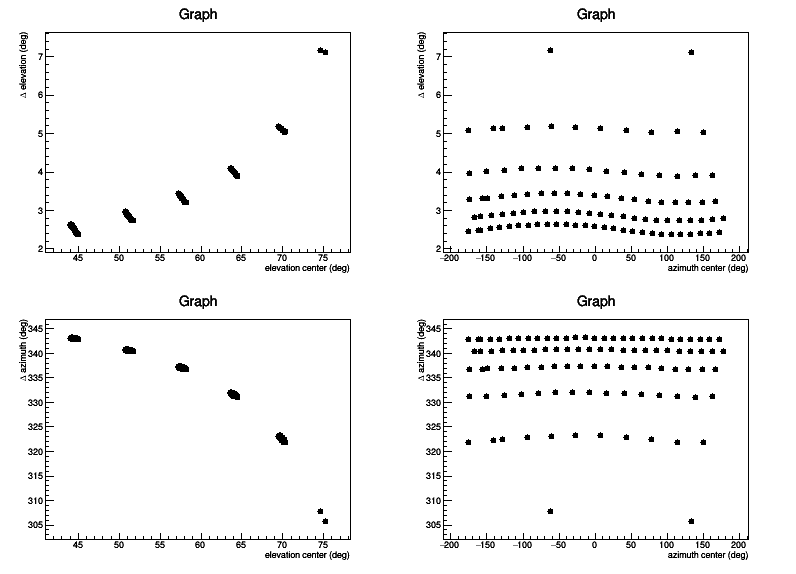
\includegraphics[width=\textwidth]{../341/data2.png}
\label{img:dataset}
\caption{Zu sehen sind die Abweichungen zwischen gemessenen und eingestellten Koordinaten in Abhängigkeit der gemessenen Koordinaten}
\end{figure}
\section{Programm}
Um das Pointingmodell auf Konsistenz zu überprüfen wurde ein Programm mit der C++ Erweiterung ROOT geschrieben, dass die optimalen Parameter für die in Kapitel \ref{ch:pointing} Pointingmodelle berechnet. Aus dem Vergleich der mit diesen Modellen vorhergesagten Werte mit den gemessenen Daten lassen sich dann Rückschlüsse über die Qualität der Pointingmodelle schließen. Nach dem Einlesen des Datensatzes wird zunächst wie oben beschrieben, ob der Pixelscale innerhalb einer Toleranz von $0,05^{\circ}$ mit dem in Tabelle \ref{tab:SkyCCD} angegebenen Wert für die Sky-CCD übereinstimmt. Um die optimalen Parameter zu finden wird die Methode der kleinsten Quadrate angewandt. Dazu werden  aus den Tupeln der Messwerte ($M_i$) und den Vorhersagen des Pointingmodells ($P_i$) mit den Parametern $\vec{q}$ Differenzen gebildet. Diese werden quadriert, damit Abweichungen nach unten den gleichen Effekt wie Abweichungen nach oben haben. Die Differenzen aller Werte des Datensatzes werden zu einer Funktion
\begin{equation}
Q(\vec{q})=\sum^N_{i=1}\left(P_i-M_i(\vec{q})\right)^2
\end{equation}
addiert, dei ein Maß für die Abweichung des Modells zu den Messwerten liefert. Diese Funktion kann mit dem eingebauten TMinuit-Paket minimiert werden um die besten Parameter des Modells zu erhalten. Um sich die zu überlegen, ob das Modell mit dem Datensatz vereinbar ist, wird die Größe $\frac{\chi^2}{doF}$ verwendet, die sich aus 
\begin{equation}
\chi^2=\sum^N_{i=1}\frac{\left(P_i-M_i\right)^2}{\sigma_i^2}
\end{equation}
und der Anzahl der Freiheitsgrade
\begin{equation}
doF=N-\textrm{Anzahl der Parameter}
\end{equation}
berechnet. Mit dem Wissen, dass der perfekte Wert für für $\frac{\chi^2}{doF}=1$ ist und der Annahme, dass alle Fehler gleich groß sind, lassen sich die Fehler wie folgt berechnen
\begin{equation}
\sigma=\sqrt{\frac{\sum^N_{i=1}\left(P_i-M_i\right)^2}{doF}}
\end{equation}
Zudem werden noch die Eigenschaften der Parameter bestimmt. Dazu wird ebenfalls mithilfe des TMinuit-Pakets die Kovarianzmatrix ausgegeben, die die Werte
\begin{equation}
COV(X,Y)=\left<\left(X-\left<X\right>\right)\cdot\left(Y-\left<Y\right>\right)\right>
\end{equation}
enthält. Auf der Hauptdiagonale stehen die Varianzen, aus denen sich die Fehler der Parameter bestimmen lassen:
\begin{equation}
\sigma_X=\sqrt{COV(X,X)}=\sqrt{VAR(X)}
\end{equation}
Interessant ist es auch, sich die Korrelation der Parameter untereinander anzusehen. Dazu wird der Korrelationskoeffizient nach Pearson $\rho$ verwendet, der ausschließlich die lineare Korrelation berücksichtigt. Für $\rho=0$ liegt keine lineare Korrelation vor und für $\rho=\pm1$ eine positive beziehungsweise eine negative lineare Korrelation. Der Korrelationskoeffizient lässt sich ebenfalls aus der Kovarianzmatrix berechnen:
\begin{equation}
\rho_{XY}=\frac{COV(X,Y)}{\sigma_X\sigma_Y}
\end{equation}
Zuletzt werden noch die Ergebnisse noch in jeweils vier Plots, die die Differenzen des Modells zu den Messwerten zeigen, graphisch dargestellt.


%Um das Pointingmodell auf Konsistenz zu überprüfen wurde ein Programm in ROOT geschrieben, welches die Differenzen der vom Pointingmodell (Index P) bestimmten Werte mit den gemessenen (Index M) Werten berechnet und analysiert. Da die oben entwickelten Pointingmodelle noch freie Parameter haben, die vom Teleskop abhängen werden diese durch eine Regression der Daten bestimmt. Da das Pointingmodell aus zwei Funktionen besteht (jeweils eine für die Elevation und den Azimut), die jedoch von den gleichen Parametern abhängen, muss hier ein kombinierter Fit durchgeführt werden. Dazu wird eine Hilfsvariable eingeführt, die die Summe der Quadrate der Differenzen von Messwerten und vorhergesagten Werten für feste Werte der freien Parameter bestimmt.
%\begin{equation}
%Q=\sum^N_{i=1}\left(P_i-M_i\right)^2
%\end{equation}
%Durch die Bildung der Quadrate können sich Abweichungen nach oben und unten nicht gegenseitig kompensieren und die Hilfsvariable ist somit ein Maß für die Abweichung von Modell mit den gewählten Parametern und Messwerten. Die besten Parameter erhält man, indem man die Variable minimiert. Dazu wurde die in ROOT integrierte Funktion TMinuit verwendet, die zudem noch die Standardabweichung der Parameter ausgibt. Um die Güte des Modells bestimmen zu können wird noch die Größe $\frac{\chi^2}{doF}$ verwendet um die Fehler der Messwerte zu bestimmen, in denen das Modell mit dem Datensatz übereinstimmt. Die Größe $\frac{\chi^2}{doF}$ ist definiert als
%\begin{equation}
%\frac{\chi^2}{doF}=\sum^N_{i=1}\frac{\left(P_i-M_i\right)^2}{\sigma_i^2}
%\end{equation}
%wobei hier $\sigma_i$ der Fehler des Wertes i ist und $doF$ der Anzahl der Freiheitsgraden entspricht. Diese berechnet sich durch
%\begin{equation}
%doF=N-\textrm{Anzahl der Parameter}
%\end{equation}
%Der perfekte Wert für $\frac{\chi^2}{doF}$ ist 1. Unter der Anahme, dass die Fehler $\sigma$ alle gleich groß sind, lassen sich diese wie folgt berechnen
%\begin{equation}
%\sigma=\sqrt{\frac{\sum^N_{i=1}\left(P_i-M_i\right)^2}{doF}}=\sqrt{\frac{Q}{doF}}
%\end{equation}
%Interessant ist es auch, sich die Korrelation der Parameter untereinander anzugucken. Die Korrelation beschreibt die Beziehung der zwischen einzelnen Parametern. Hier wird dazu der Korrelationskoeffizient nach Pearson verwendet, der ausschließlich die lineare Korrelation berücksichtigt. Um diesen zu berechnen wird zunächst die Korelationsmatrix
%\begin{equation}
%COV(X,Y)=\left<\left(X-\left<X\right>\right)\cdot\left(Y-\left<Y\right>\right)\right>
%\end{equation}
%berechnet. Auf der Hauptdiagonale stehen die Varianzen, aus denen sich die Fehler der Parameter bestimmen lassen:
%\begin{equation}
%\sigma_X=\sqrt{COV(X,X)}=\sqrt{VAR(X)}
%\end{equation}
%Der Korrelationskoeffizient lässt sich nun durch
%\begin{equation}
%\rho_{XY}=\frac{COV(X,Y)}{\sigma_X\sigma_Y}
%\end{equation}\\
%Um die Qualität der jeweiligen Pointingmodelle beurteilen zu können, werden jeweils vier Plots ausgegeben, die die jeweiligen Differenzen der bestimmten und gemessenen Koordinaten angeben
%\begin{equation}
%f=el_M-el_P \quad \textrm{bzw} \quad f=az_M-az_P
%\end{equation}
\section{Anwendung auf das Pointingmodell mit 2 Parametern}
Zunächst wird das Modell mit den Parametern $el_0$ und $az_0$ untersucht.
\subsection{Abhängigkeit der Drivekoordinaten in Abhängigkeit der CCD-Koordinaten}
Um die Koordinaten des Teleskops anhand der Koordinaten der CCD-Kamera vorherzusagen wird das Modell aus den Gleichungen \ref{eq:elC2D} und \ref{eq:azC2D} verwendet. Berechnet man die Parameter mit dem oben beschriebenen Programm so erhält man die Parameter in Tabelle \ref{tab:C2D}. Die Abweichungen zwischen Vorhersage und gemessenen Werten sind in Abbildung \ref{img:C2D} zu sehen.
\begin{figure}[htbp]
\centering
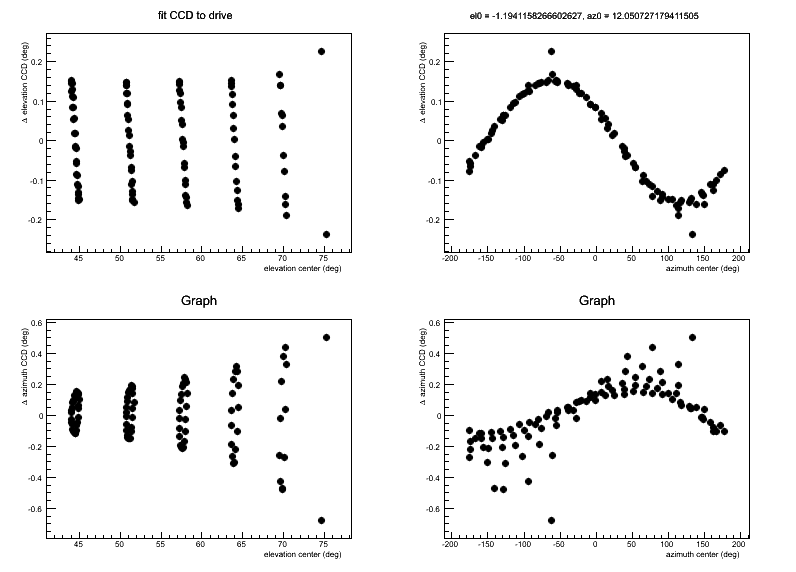
\includegraphics[width=\textwidth]{../341/run341C2D.png}
\caption{Die Drivekoordinaten in Abhängigkeit der CCD-Koordinaten}
\label{img:C2D}
\end{figure}

\begin{table}[htbp]
\centering
\begin{tabular}{rcl}
\toprule
$el0$ &=& $(-1,1941\pm0,0098)^{\circ}$\\
$az0$ &=& $(12,0507\pm0,0019)^{\circ}$\\
$\sigma$ &=& $0,23^{\circ}$\\
$\rho_{el_0,az0}$ &=& $0,1576$\\
\bottomrule
\end{tabular}
\label{tab:C2D}
\caption{Die für das Pointingmodell mit 2 Parametern bestimmten Werte}
\end{table}

\subsection{Abhängigkeit der CCD-Koordinaten in Abhängigkeit der Drivekoordinaten}
Für das inverse Modell werden die Gleichungen \ref{eq:elD2C} und \ref{eq:azD2C} verwendet. Mit diesen kommt man auf die Werte in Tabelle \ref{tab:D2C} und die in Abbildung \ref{img:D2C} gezeigten Abbildungen.
\begin{figure}[htbp]
\centering
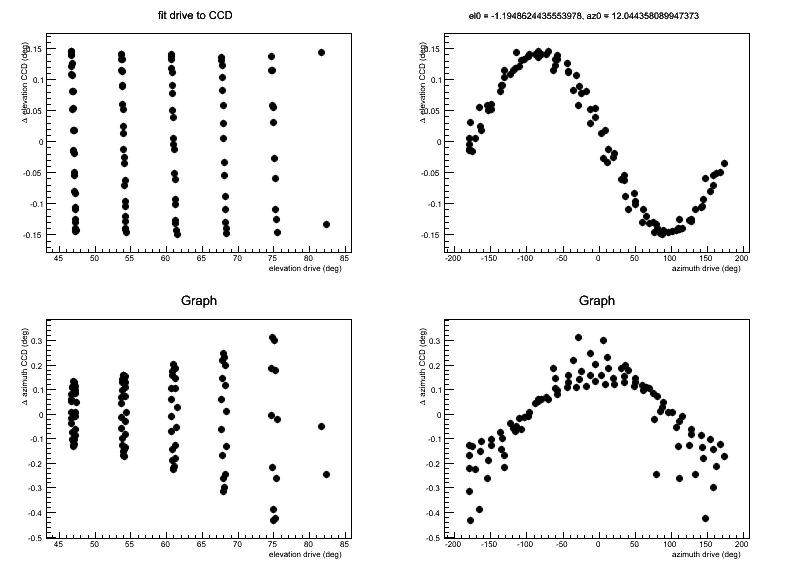
\includegraphics[width=\textwidth]{../341/run341D2C.png}
\caption{Die CCD-Koordinaten in Abhängigkeit der Driveoordinaten im Zwei-Parameter-Modell}
\label{img:D2C}
\end{figure}

\end{figure}
\begin{table}[htbp]
\centering
\begin{tabular}{rcl}
\toprule
$el0$ &=& $(-1,184\pm0,008)^{\circ}$\\
$az0$ &=& $(12,048\pm0,004)^{\circ}$\\
$\sigma$ &=& $0,19^{\circ}$\\
$\rho_{el_0,az0}$ &=& $-0,4698$\\
\bottomrule
\end{tabular}
\label{tab:D2C}
\caption{Die Drive-Koordinaten in Abhängigkeit der CCD-Koordinaten im Zwei-Parameter-Modell}
\end{table}

\section{Anwendung auf das Pointingmodell mit 4 Parametern}
Im folgenden wird das obige Modell auf vier Parameter erweitert indem wie in Abschnitt \ref{se:4par} beschrieben jeweils ein konstanter Wert zu den Drive-Koordinaten hinzuaddiert wird.
\subsection{Abhängigkeit der Drivekoordinaten in Abhängigkeit der CCD-Koordinaten}
Werden die Formeln \ref{eq:elC2D4} und \ref{eq:azC2D4} verwendet erhält man die in Abbildung \ref{img:C2D4} gezeigten Differenzen und die in Tabelle \ref{tab:C2D4} aufgelisteten Werte.
\begin{figure}[htbp]
\centering
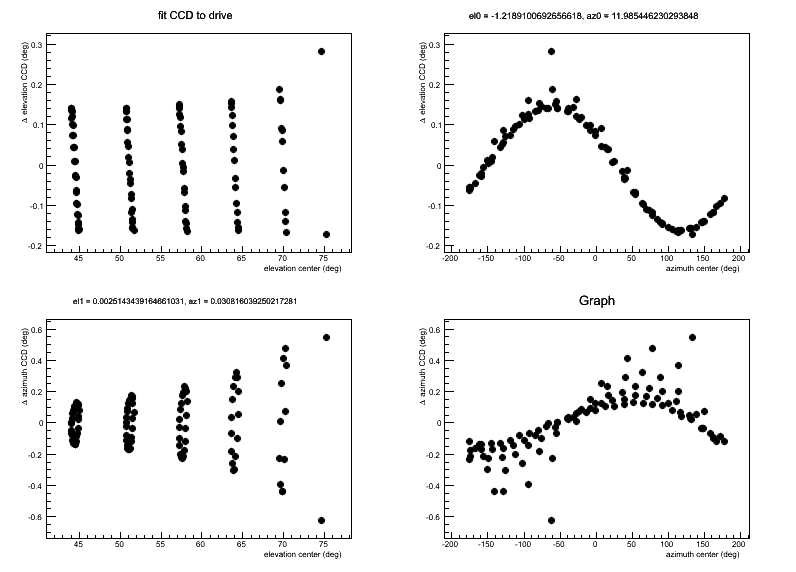
\includegraphics[width=\textwidth]{../341/run341C2D_4par.png}
\caption{Die Drivekoordinaten in Abhängigkeit der CCD-Koordinaten}
\label{img:C2D4}
\end{figure}
\begin{table}[htbp]
\centering
\begin{tabular}{rcl}
\toprule
$el0$ &=& $(-1,21891\pm 0,03924)^{\circ}$\\
$az0$ &=& $(11,9854\pm0,2072)^{\circ}$\\
$el_1$ &=& $(0,00251434\pm 0,0001839)^{\circ}$\\
$az0$ &=& $(0,03080816\pm0,2149)^{\circ}$\\
$\sigma$ &=& $0,23^{\circ}$\\
$\rho_{el_0,az_0}$ &=& $0,8691$\\
$\rho_{el_0,el_1}$ &=& $-0,8417$\\
$\rho_{az_0,az_1}$ &=& $-0,9358$\\
$\rho_{el_0,az_1}$ &=& $-0,8137$\\
$\rho_{az_0,el_1}$ &=& $-0,9709$\\
$\rho_{el_1,el_1}$ &=& $-0,8417$\\
\bottomrule
\end{tabular}
\label{tab:C2D4}
\caption{Die für das Pointingmodell mit 4 Parametern bestimmten Werte}
\end{table}

\subsection{Abhängigkeit der CCD-Koordinaten in Abhängigkeit der Drivekoordinaten}
Invertiert man das Modell, so verwendet man die Gleichungen \ref{eq:elD2C4} und \ref{eq:azD2C4}, sodass das das Programm die Werte aus Tabelle \ref{tab:D2C4} und die Abstände aus Abbildung \ref{img:D2C4} liefert.
\begin{figure}[htbp]
\centering
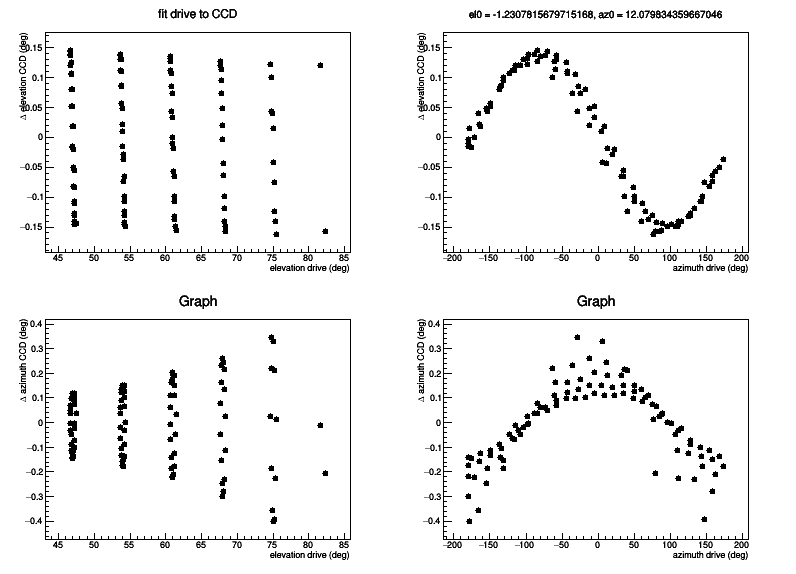
\includegraphics[width=\textwidth]{../341/run341D2C4.png}
\caption{Die CCD-Koordinaten in Abhängigkeit der Driveoordinaten}
\label{img:D2C4}
\end{figure}
\begin{table}[htbp]
\centering
\begin{tabular}{rcl}
\toprule
$el0$ &=& $(-1,19373\pm 0,9976)^{\circ}$\\
$az0$ &=& $(12,0957\pm0,04068)^{\circ}$\\
$el_1$ &=& $(0,0192352\pm 1,043)^{\circ}$\\
$az0$ &=& $(-0,0946443\pm0,1452)^{\circ}$\\
$\sigma$ &=& $0,10^{\circ}$\\
$\rho_{el_0,az_0}$&=& $-0,009202$\\
$\rho_{el_0,el_1}$&=& $-0,0218$\\
$\rho_{az_0,az_1}$&=& $-0,9493$\\
$\rho_{el_0,az_1}$&=& $-0,9954$\\
$\rho_{az_0,el_1}$&=& $-0,03329$\\
$\rho_{el_1,el_1}$&=& $-0,01867$\\
\bottomrule
\end{tabular}
\label{tab:D2C4}
\caption{Die für das Pointingmodell mit 4 Parametern bestimmten Werte}
\end{table}

\section{Diskussion der Korrelation}
Sieht man sich die einzelnen Korrelationen an, so erkennt man, dass sich diese für das jeweils gleiche Modell mit gleich vielen Parametern stark unterscheiden und gerade im Modell mit vier Parametern sehr starke Korrelationen auftreten.
\subsection{Unterschiedliche Korrelationen für Modelle mit gleichen Parametern}
Zunächst fällt auf, dass sich im Modell mit zwei Parametern die Korrelationskoeffizienten stark unterscheiden
\subsection{Hohe Korrelation im Modell mit vier Parametern}

\section{Systematische Abweichungen im entwickelten Pointingmodell}
